\documentclass[tikz,border=3pt]{standalone}
\usepackage[utf8]{inputenc}
\usepackage[T1]{fontenc}
\usepackage{lmodern}
\renewcommand{\familydefault}{\sfdefault}
\usepackage{sansmath}\sansmath
\usepackage{chemfig}
\usepackage{pgfplots}\pgfplotsset{compat=1.18,/pgf/number format/use comma,/pgf/number format/1000 sep={.}}
\usetikzlibrary{arrows.meta,calc,positioning,decorations.pathmorphing,patterns}
% paleta del sitio
\definecolor{nar}{HTML}{E8680C}\definecolor{narc}{HTML}{FFB35C}\definecolor{hielo}{HTML}{FFF3E8}
\definecolor{tinta}{HTML}{1D1D1F}\definecolor{gris}{HTML}{6E6E73}\definecolor{lila}{HTML}{7C5CF0}
\definecolor{azul}{HTML}{2F6FD6}\definecolor{menta}{HTML}{17A673}\definecolor{coral}{HTML}{E8342A}
\begin{document}
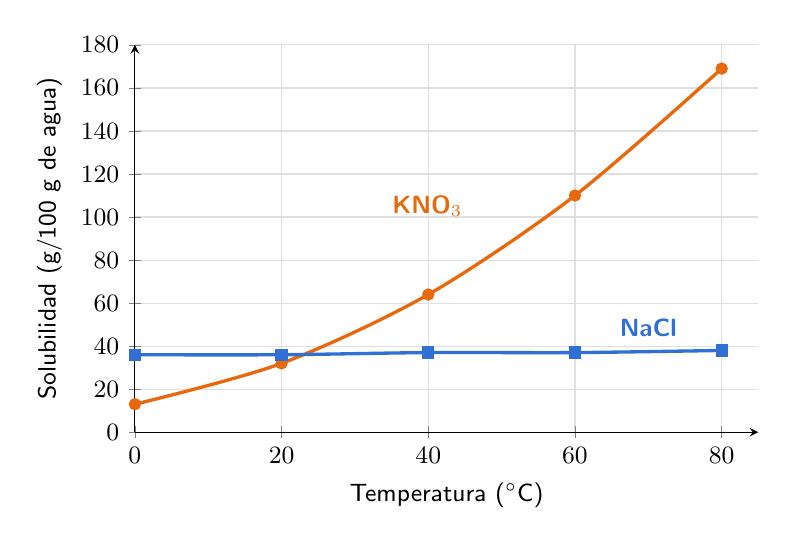
\begin{tikzpicture}[font=\small]
\begin{axis}[width=9.5cm,height=6.5cm,axis lines=left,xmin=0,xmax=85,ymin=0,ymax=180,xtick={0,20,40,60,80},ytick={0,20,40,60,80,100,120,140,160,180},
  grid=major,grid style={gray!25},xlabel={Temperatura ($^\circ$C)},ylabel={Solubilidad (g/100 g de agua)},clip=false]
\addplot[nar,very thick,smooth,mark=*,mark options={fill=nar,scale=0.8}] coordinates {(0,13)(20,32)(40,64)(60,110)(80,169)};
\addplot[azul,very thick,smooth,mark=square*,mark options={fill=azul,scale=0.8}] coordinates {(0,36)(20,36)(40,37)(60,37)(80,38)};
\node[nar,font=\small\bfseries,anchor=east] at (axis cs:46,105) {KNO$_3$};
\node[azul,font=\small\bfseries,anchor=south] at (axis cs:70,40) {NaCl};
\end{axis}
\end{tikzpicture}
\end{document}
